%
% fig-polargeodaete.tex
%
% (c) 2025 Prof Dr Andreas Müller
%
\begin{figure}
\centering
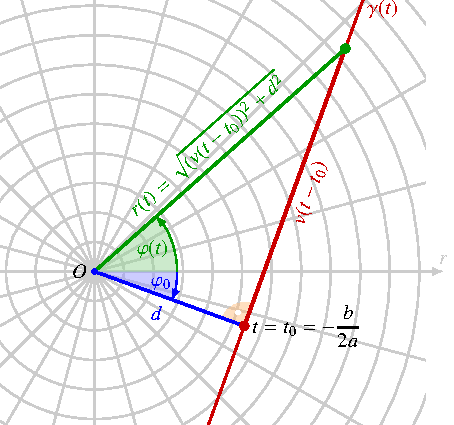
\includegraphics{chapters/100-zusammenhang/images/polargeodaete.pdf}
\caption{Geodäten in Polarkoordinaten sind Geraden.
Der Radius in Abhängigkeit vom Parameter ist $r(t)$, die Gerade
geht für den Parameterwert $t_0=-b/2a$ im kleinsten Abstand $d$
am Nullpunkt vorbei.
\label{buch:zusammenhang:geodaeten:fig:polargeodaete}}
\end{figure}
